\documentclass[10pt, a4paper]{book}

\hbadness = \maxdimen
\vbadness = \maxdimen

\usepackage[utf8]{inputenx}
\usepackage[brazil]{babel}
\usepackage{textcomp}
\usepackage{float}
\usepackage{amsfonts, mathtools}

\usepackage{caption}	
	\DeclareCaptionLabelSeparator{dash}{ -- }
	\captionsetup{
		labelfont = {sf, bf},
		labelsep = dash,
		size = footnotesize,
		width=0.9\textwidth
	}

\usepackage{graphicx}
\graphicspath{{Figuras/}}

\usepackage[margin=3cm]{geometry}
\usepackage{fancyhdr, lastpage}
\renewcommand{\footrulewidth}{0.5pt}
\pagestyle{fancy}
\fancyhf{}
\fancyhead[LE,RO]{\rightmark}
\fancyhead[RE,LO]{\leftmark}
\fancyfoot[L]{Técnicas não lineares em Controle}
\fancyfoot[R]{\thepage/\pageref{LastPage}}

\usepackage{tikz}

\usepackage{titlesec}
\titleformat{\section}
{\normalfont\Large\bfseries}{\thesection}{1em}{}%
[\vskip-25pt\hskip-90pt\begin{tikzpicture}
	\fill [teal, opacity=0.2, rounded corners=5pt] 
		(0,0) rectangle (6.12, 1) 
	;
\end{tikzpicture}]

\usepackage{amsmath, amsthm, amssymb}
	\renewcommand{\bar}{\overline}
	\newcommand{\del}{\partial}
	\newcommand{\I}{\mathbb{I}}
	\newcommand{\R}{\mathbb{R}}
	\newcommand{\e}{\varepsilon}
	\renewcommand{\leq}{\leqslant}
	\renewcommand{\geq}{\geqslant}
	\newcommand{\dis}{\displaystyle}
	\renewcommand{\Re}{\mathrm{Re}}
	\renewcommand{\Im}{\mathrm{Im}} % ainda não foi usado

\usepackage{xcolor, listings}
\definecolor{codegreen}{rgb}{0,0.6,0}
\definecolor{codegray}{rgb}{0.5,0.5,0.5}
\definecolor{codepurple}{rgb}{0.58,0,0.82}
% Python
\lstset{
	language = Python,
	commentstyle=\color{codegreen},
	keywordstyle=\color{codepurple},
	stringstyle=\color{orange!70!black},
	basicstyle=\linespread{1}\ttfamily\small,
	numberstyle=\footnotesize,
	numbers=left,
	backgroundcolor=\color{gray!10},
	frame=single,
	tabsize=2,
	rulecolor=\color{black!30},
	title=\lstname,
	escapeinside={\%*}{*)},
	breaklines=true,
	breakatwhitespace=true,
	framextopmargin=2pt,
	framexbottommargin=2pt,
	extendedchars=true,
	inputencoding=utf8,
	literate={á}{{\'a}}1 {ã}{{\~a}}1 {é}{{\'e}}1 {ç}{{\c{c}}}1 {â}{{\^a}}1 {õ}{{\~o}}1 {ú}{{\'u}}1 {ó}{{\'o}}1 {í}{{\'i}}1 {Í}{{\'I}}1 
}

\usepackage[hidelinks]{hyperref}


\begin{document}
	% capa
	\thispagestyle{empty}
	\begin{tikzpicture}[remember picture, overlay]
		\node at (current page.center) {
			
\includegraphics{Figuras/capa tnlc.pdf}
		};
	\end{tikzpicture}
	
	\clearpage
	\pagenumbering{arabic}
	\section*{24/06/2022 --- Pontos de Equilíbrio e Linearização}
\markboth{Pontos de Equilíbrio e Linearização}{24/06/2022}
\noindent\textbf{\sffamily Exercício 1.}
\begin{itemize}
	\item [a)] 
	Determine os pontos de equilíbrio do sistema abaixo.
	
	\item [b)] 
	Determine o sistema linearizado tangente de cada ponto de equilíbrio e analise sua instabilidade.
\end{itemize}
%
\[
\frac{d^2\theta}{dt^2} = 
\theta^2 - 2\theta - 10\frac{d\theta}{dt} 
\]
%

\noindent\textbf{\sffamily Exercício 2.}
\begin{itemize}
	\item [a)] 
	Determine os pontos de equilíbrio do sistema abaixo.
	
	\item [b)] 
	Determine o sistema linearizado tangente de cada ponto de equilíbrio e analise sua instabilidade.
\end{itemize}
%
\begin{align*}
	\frac{d\theta_1}{dt} &= 
	\theta_1^2 - 2\theta_2\theta_1 - u \\
	%
	\frac{d\theta_2}{dt} &= 
	\theta_1 -3\theta_2 + 2\sin\theta_2 + u\theta_2
\end{align*}
%
\rule{\textwidth}{0.5pt}


\noindent
\textbf{\sffamily Exercício 1 --- solução.}
\begin{itemize}
	\item [a)] 
	Primeiro definimos as equações de estado. 
	Pondo 
	$x_1 = \theta$ e 
	$x_2 = \dot{\theta}$, temos 
	%
	\begin{align*}
		\dot{x}_1 &= x_2 \\
		\dot{x}_2 &= x_1^2 - 2x_1 - 10x_2  
	\end{align*}
	%
	Seja $(\bar{x_1}, \bar{x_2})$ um ponto de equilíbrio. Por definição,
	%
	\begin{align*}
		\begin{array}{l}
			0 = \bar{x_2} \\
			0 = \bar{x_1}^2 - 2\bar{x_1} - 10\bar{x_2} 
		\end{array} 
		\quad\iff\quad 
		\bar{x_1} = 0 \text{ ou } \bar{x_1}=2, \quad 
		\bar{x_2} = 0.
	\end{align*}
	%
	Logo, os pontos de equilíbrio são 
	$P_1 = (0, 0)$ e 
	$P_2 = (2, 0)$.
	%		
	
	\item [b)] 
	Apenas a segunda equação de estado precisa ser linearizada 
	(como é possível tomar $y=x_1-\bar{x_1}$, a saída também não precisará ser linearizada).
	Temos 
	%
	\begin{align*}
		\dot{x}_2 = f_2(x_1, x_2) 
		&\approx f_2(\bar{x_1}, \bar{x_2}) 
		+
		\del_{x_1} f_2\bigg|_{\bar{x_1}, \bar{x_2}}
		(x_1 - \bar{x_1}) 
		+
		\del_{x_2} f_2\bigg|_{\bar{x_1}, \bar{x_2}}
		(x_2 - \bar{x_2}) \\
		&= (2\bar{x_1} - 2)(x_1 - \bar{x_1}) -
		10x_2,
	\end{align*}
	%
	e daí, pela mudança de variável 
	$x_1-\bar{x_1} \rightarrow x_1$, o sistema linearizado é  
	%
	\begin{align*}
		\begin{array}{l}
			\dot{x}_1 = x_2 \\
			\dot{x}_2 =(2\bar{x_1} - 2)(x_1 - \bar{x_1}) - 10x_2 
		\end{array}
		\quad \iff \quad 
		\begin{pmatrix}
			\dot{x}_1 \\ \dot{x}_2
		\end{pmatrix}
		&= 
		\begin{pmatrix}
			0 & 1 \\
			2\bar{x_1} - 2 & -10 
		\end{pmatrix}
		\begin{pmatrix}
			x_1 - \bar{x_1} \\ x_2 - \bar{x_2}
		\end{pmatrix},
		\\
		y&= \begin{pmatrix} 1 & 0 \end{pmatrix} 
		\begin{pmatrix} x_1 \\ x_2 \end{pmatrix}.
	\end{align*}
	%
	Considerando os valores dos pontos de equilíbrio, temos
	%
	\begin{align*}
		P_1 \implies 
		\dot{X} &= 
		\begin{pmatrix}
			0 & 1 \\
			- 2 & -10 
		\end{pmatrix}
		X, \\
		P_2 \implies 
		\dot{X} &= 
		\begin{pmatrix}
			0 & 1 \\
			2 & -10
		\end{pmatrix}
		\begin{pmatrix}
			x_1-2 \\ x_2
		\end{pmatrix}
	\end{align*}
	%
\end{itemize}
%

\clearpage
\noindent
\textbf{\sffamily Exercício 2 --- solução.}
\begin{itemize}
	\item [a)] 
	Seja $(\bar{\theta_1}, \bar{\theta_2})$ um ponto de equilíbrio. Então,
	%
	\[
	\begin{array}{l}
		0 = 
		\bar{\theta_1}^2 - 2\bar{\theta_2}\cdot \bar{\theta_1} - 0 \\
		%
		0 = 
		\bar{\theta_1} -3\bar{\theta_2} + 2\sin\bar{\theta_2} + 0
	\end{array}
	\implies
	\begin{array}{l}
		0 = 
		\bar{\theta_1}(\bar{\theta_1} - 2\bar{\theta_2}) \\
		%
		0 = 
		\bar{\theta_1} -3\bar{\theta_2} + 2\sin\bar{\theta_2}
	\end{array}.
	\]
	%
	Pela primeira equação acima, ou 
	$\bar{\theta_1}=0$ ou 
	$\bar{\theta_1} - 2\bar{\theta_2}=0$.
	Assumindo o primeiro caso, é imediato pela segunda equação que 
	$\sin\bar{\theta_2}=1,5\bar{\theta_2}$. 
	A série de Taylor do seno ao redor da origem nos diz que a única solução dessa equação é $\bar{\theta_2}=0$. 
	Por outro lado, assumindo $\bar{\theta_1}=2\bar{\theta_2}$, encontramos que 
	$\sin\bar{\theta_2} = 0,5\bar{\theta_2}$, que, novamente pela série de Taylor, possuirá 3 soluções. 
	Por auxílio de uma calculadora gráfica, as raízes são 
	$\bar{\theta_2} = 0$ (de novo),
	$\bar{\theta_2} \approx \pm 1,895$.
	Os pontos de equilíbrio ficam então 
	%
	\[
	P_1 = \begin{pmatrix} 0 \\ 0 \end{pmatrix}, \quad 
	P_2 = \begin{pmatrix} 3,79 \\ 1,895 \end{pmatrix}, \quad 
	P_3 = \begin{pmatrix} -3,79 \\ -1,895 \end{pmatrix}.
	\]
	%
	\begin{figure}[h!]\centering
		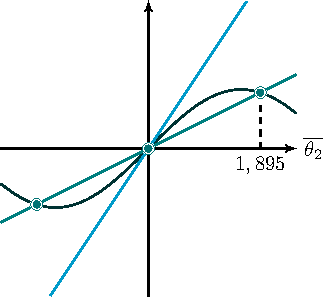
\includegraphics{em busca de theta2.pdf}
		\caption{%
			Gráficos em escala das funções $\sin\bar{\theta_2}$, 
			$0,5\bar{\theta_2}$, e
			$1,5\bar{\theta_2}$.
			Destaque para os pontos de interseção.
		}
	\end{figure}
	
	\item [b)] 
	Ambas equações de estado precisam ser linearizadas. 
	Temos 
	%
	\begin{align*}
		\dot{\theta}_1 = f_1(\theta_1, \theta_2; u)
		&\approx f_1(\bar{\theta_1}, \bar{\theta_2}; u) 
		+
		\del_{\theta_1} f_1
		\bigg|_{\bar{\theta_1}, \bar{\theta_2}}
		(\theta_1 - \bar{\theta_1}) 
		+
		\del_{\theta_2} f_1
		\bigg|_{\bar{\theta_1}, \bar{\theta_2}}
		(\theta_2 - \bar{\theta_2}) 
		+
		\del_{u} f_1
		\bigg|_{\bar{\theta_1}, \bar{\theta_2}}
		u 
		\\
		&= (2\bar{\theta_1} - 2\bar{\theta_2})(\theta_1 - \bar{\theta_1})
		-2\bar{\theta_2}(\theta_2 - \bar{\theta_2})
		-u, 
		\\
		\dot{\theta}_2 = f_2(\theta_1, \theta_2; u)
		&\approx f_2(\bar{\theta_1}, \bar{\theta_2}; u) 
		+
		\del_{\theta_1} f_2
		\bigg|_{\bar{\theta_1}, \bar{\theta_2}}
		(\theta_1 - \bar{\theta_1}) 
		+
		\del_{\theta_2} f_2
		\bigg|_{\bar{\theta_1}, \bar{\theta_2}}
		(\theta_2 - \bar{\theta_2}) 
		+
		\del_{u} f_2
		\bigg|_{\bar{\theta_1}, \bar{\theta_2}}
		u  
		\\
		&= (\theta_1 - \bar{\theta_1})+
		(-3-2\cos\bar{\theta_2})(\theta_2 - \bar{\theta_2})
		+\bar{\theta_2}u, 
	\end{align*}
	%
	e portanto
	%
	\[
	\begin{pmatrix}
		\dot{\theta}_1 \\ \dot{\theta}_2
	\end{pmatrix}
	= 
	\begin{pmatrix}
		2\bar{\theta_1} - 2\bar{\theta_2} & -2\bar{\theta_2} \\
		1 & -3+2\cos\bar{\theta_2} 
	\end{pmatrix}
	\begin{pmatrix}
		\theta_1 - \bar{\theta_1} \\ \theta_2 - \bar{\theta_2}
	\end{pmatrix}
	+
	\begin{pmatrix}
		-1 \\ \bar{\theta_2}
	\end{pmatrix},
	u
	\]
	%
	de forma que
	%
	\begin{align*}
		P_1 \implies \dot{\Theta} &= 
		\begin{pmatrix} 
			0 & 0 \\ 
			1 & -1
		\end{pmatrix}
		\Theta 
		+
		\begin{pmatrix} -1 \\ 0 \end{pmatrix} u, \\
		P_2 \implies \dot{\Theta} &=
		\begin{pmatrix} 
			3,79 & -7,58 \\ 
			1 & -1,001
		\end{pmatrix}
		\begin{pmatrix}
			\theta_1 - 3,79 \\
			\theta_2 - 1,895
		\end{pmatrix}
		+
		\begin{pmatrix} -1 \\ 1,895 \end{pmatrix} u, \\
		P_3 \implies \dot{\Theta} &=
		\begin{pmatrix} 
			-3,79 & 7,58 \\ 
			1 & -1,001
		\end{pmatrix}
		\begin{pmatrix}
			\theta_1 + 3,79 \\
			\theta_2 + 1,895
		\end{pmatrix}
		+
		\begin{pmatrix} -1 \\ -1,895 \end{pmatrix} u.
	\end{align*}
\end{itemize}
%	
	\section*{01/07/2022 --- Retrato de fase e critério de Lyapunov}
\markboth{Retrato de fase e critério de Lyapunov}{01/07/2022}
\noindent\textbf{\sffamily Exercício 1.}
	Desenhe e classifique o retrato de fase do sistema descrito por 
	%
	\begin{align*}
		\dot{x}_1 &= -x_1 + x_2 \\
		\dot{x}_2 &= -0,5x_1 -3x_2
	\end{align*}
	
	\noindent\textbf{\sffamily Exercício 2.}
	Desenhe e classifique o retrato de fase do sistema descrito por 
	%
	\begin{align*}
		\dot{x}_1 &= -2x_1 - 4x_2 \\
		\dot{x}_2 &= -4x_1 -2x_2
	\end{align*}
	
	\noindent\textbf{\sffamily Exercício 3.}
	Desenhe e classifique o retrato de fase do sistema descrito por 
	%
	\begin{align*}
		\dot{x}_1 &= x_2 \\
		\dot{x}_2 &= (1-x_1^2)x_2 - x_1
	\end{align*}
	%
	chamado \emph{equação de Van der Pol}. \\
	
	\noindent\textbf{\sffamily Exercício 4.} \\
	Verifique que o sistema massa mola sem atrito é estável pela função de Lyapunov 
	$H(x) = \frac{m\dot{x}^2}{2} + \frac{kx^2}{2}$ (energia do sistema). \\
	
	\noindent\textbf{\sffamily Exercício 5.} \\
	Verifique que o sistema massa mola com atrito viscoso é assintoticamente estável pela função de Lyapunov 
	$H(x) = \frac{m\dot{x}^2}{2} + \frac{kx^2}{2}$. \\
	%
	\rule{\textwidth}{0.5pt} 
	%	
	
	\noindent
	\textbf{\sffamily Exercício 1 --- solução.} \\
	O sistema linear tem único ponto de equilíbrio em $(0,0)$. 
	Calculando os autovalores, temos 
	%
	\begin{align*}
		\det(\lambda\I - A) = 0 \implies
		\det
		\begin{pmatrix}
			\lambda+1 & -1 \\
			0,5 & \lambda+3
		\end{pmatrix}
		&= 0 \\
		\iff
		(\lambda+1)(\lambda+3) + \frac{1}{2} &= 0 
		\implies 
		\lambda = -2 \pm \frac{1}{\sqrt{2}}
	\end{align*}
	% 
	Como os autovalores são reais negativos distintos, $(0,0)$ será um nó estável do retrato de fase. 
	Além disso, temos autovetores lento $v_s$ e rápido $v_f$ dados por 
	%
	\begin{align*}
		Av_s &= \left(-2+\frac{1}{\sqrt{2}}\right) v_s \iff 
		v_s = \alpha \binom{1}{\frac{1}{\sqrt{2}}-1},
		\\
		Av_f &= \left(-2-\frac{1}{\sqrt{2}}\right) v_f \iff 
		v_f = \beta \binom{1}{-\frac{1}{\sqrt{2}}-1} 
		.
	\end{align*}
	% 
	Logo as trajetórias no retrato partem de retas paralelas a $v_f$ em direção à origem pela reta formada por $v_s$.
	Confira o retrato na figura a seguir, gerada através do código abaixo.
	%
	\begin{figure}[H]\centering
		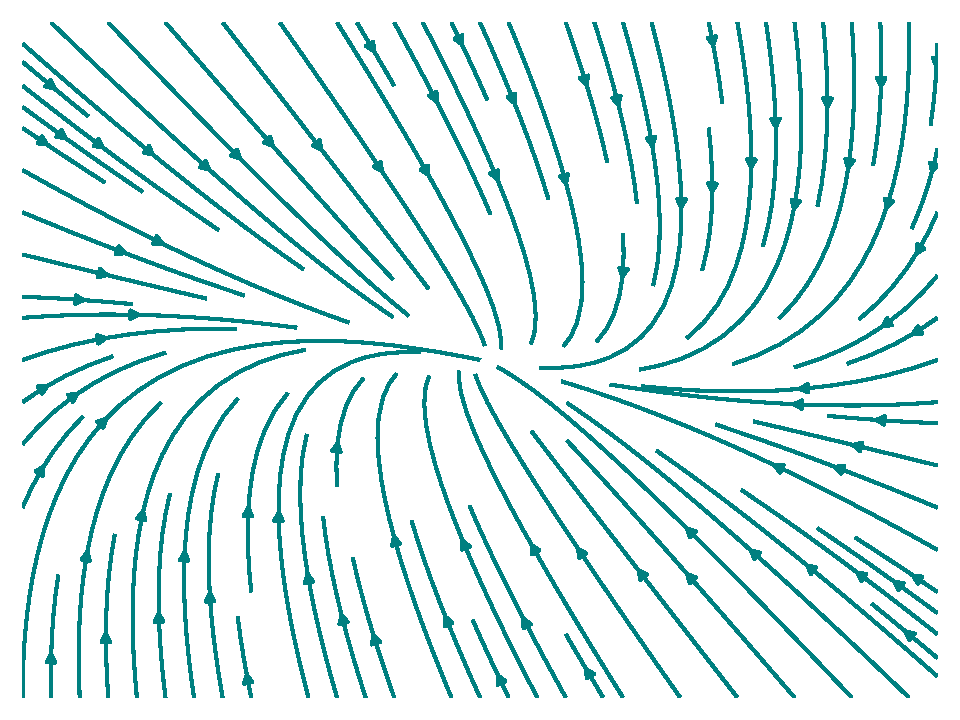
\includegraphics[width=7cm]{nó estável.pdf} 
	\end{figure}
	%
	\lstinputlisting[language=Python, caption=Código Python para ilustrar o retrato de fase]{phase portrait.py}
	
	\noindent
	\textbf{\sffamily Exercício 2 --- solução.} \\
	O ponto de equilíbrio é novamente o $(0,0)$. 
	Na verdade, este é o equilíbrio em todos os exercícios.
	Calculando os autovalores, temos
	%
	\begin{align*}
		\det(\lambda\I - A) = 0 \implies
		\det
		\begin{pmatrix}
			\lambda+2 & 4 \\
			4 & \lambda+2
		\end{pmatrix}
		&= 0 \\
		\iff
		(\lambda+2)(\lambda+2) - 16 &= 0 
		\implies 
		\lambda = -2 \pm 4,
	\end{align*}
	%
	isto é, autovalores de sinais distintos. 
	Isso mostra que a origem é ponto de sela do retrato, e a próxima tarefa é encontrar as direções (autovetores) de divergência ($v_d$) e convergência ($v_c$) por esse ponto. 
	Daí,
	%
	\begin{align*}
		Av_d = 2v_d \iff v_d = \alpha\binom{1}{-1} ,
		\quad
		Av_c = 2v_c \iff v_c = \alpha\binom{1}{1} . 
	\end{align*}
	%
	O retrato fica
	%
	\begin{figure}[H]\centering
		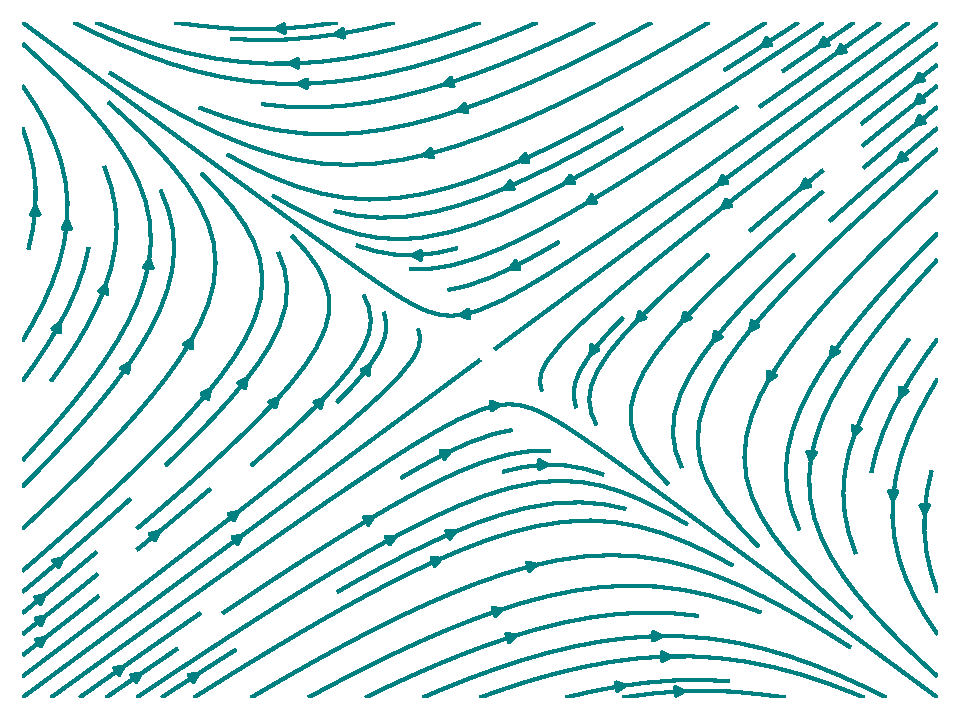
\includegraphics[width=7cm]{sela.pdf} 
	\end{figure}
	%
	
	\noindent
	\textbf{\sffamily Exercício 3 --- solução.} \\
	Ao contrário dos exercícios anteriores, estas EDs não são lineares, e o que buscaremos achar é apenas uma tentativa de aproximação local na origem. 
	Linearizando nessa região, 
	%
	\begin{align*}
		\dot{X} \approx 
		\begin{pmatrix}
			0 & 1 \\
			-1 - 2\bar{x_1}\bar{x_2} & 1-\bar{x_1}^2
		\end{pmatrix}
		X
		=
		\begin{pmatrix}
			 0 & 1 \\
			-1 & 1
		\end{pmatrix}
		X,
	\end{align*}
	%
	e segue daí que¨
	%
	\begin{align*}
		\det(\lambda\I - A) = 0 \implies 
		\det
		\begin{pmatrix}
			\lambda & -1 \\
			1 & \lambda-1
		\end{pmatrix}
		&= 0 \\
		\iff
		\lambda(\lambda-1) + 1 &= 0
		\implies 
		\lambda = \frac{1}{2} \pm i\frac{\sqrt{3}}{2}.
	\end{align*}
	%
	Como os autovalores têm parte real positiva e parte imaginária não nula, trata-se de um foco instável. 
	O interessante da equação de Van der Pol, entretanto, é que para $x_1$ suficientemente grade, o sistema deixa de divergir e ``entra em loop"; 
	em outras palavras, a instabilidade do foco pode levar o sistema a um comportamento oscilatório. 
	Vide o retrato a seguir.
	%
	\begin{figure}[H]\centering
		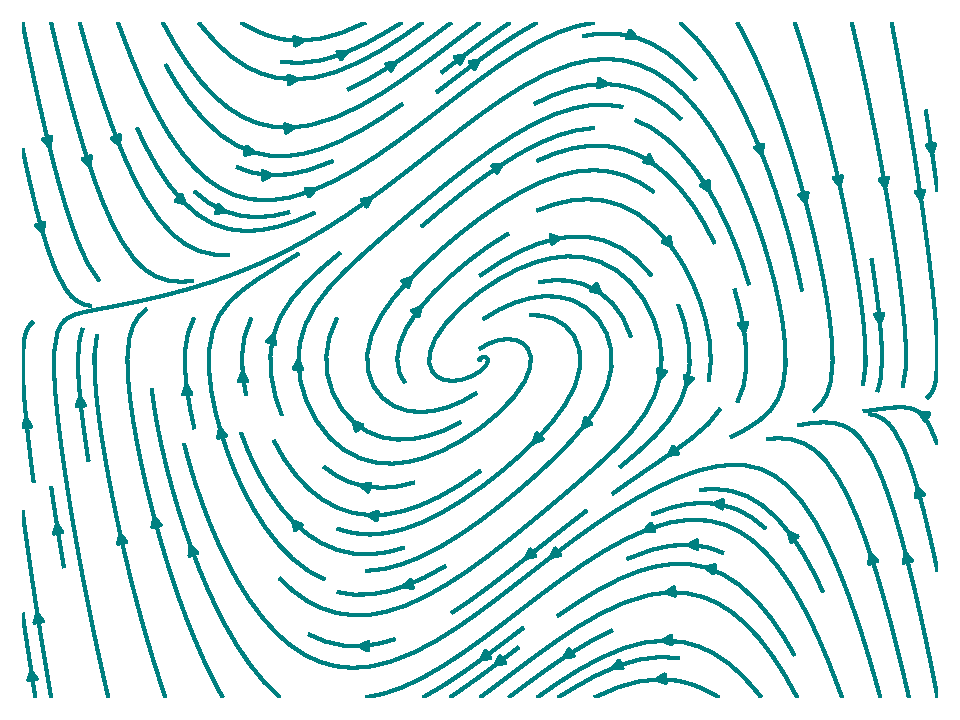
\includegraphics[width=7cm]{van der pol.pdf}
	\end{figure}
	%
	
	\noindent
	\textbf{\sffamily Exercício 4 --- solução.} \\
	Em outras palavras, queremos verificar que 
	$H(x)\geq 0$, 
	$H(\bar{x})=0$ e 
	$\dot{H}(x(t)) \leq 0$ para a EDO massa-mola 
	%
	\[
		m\ddot{x} + kx = 0.
	\]
	%
	As primeiras duas igualdades são triviais; quanto à última, temos 
	%
	\begin{align*}
		\dot{H} &= \frac{d}{dt} \left(
		               \frac{m\dot{x}^2}{2} + 
		               \frac{kx^2}{2}
		           \right) \\
		        &= \frac{m}{2} (2\dot{x}\ddot{x}) +
		           \frac{k}{2} (2x\dot{x}) \\
		        &= \dot{x}
		           \underbrace{(m\ddot{x} + kx)}_{=0} 
		        \equiv 0.
	\end{align*} 
	%
	Logo o sistema é de fato estável e $H$ é uma função de Lyapunov. \\
	%
	
	\noindent
	\textbf{\sffamily Exercício 5 --- solução.} \\
	Desta vez, tratamos do sistema 
	%
	\[
		m\ddot{x} + \alpha \dot{x}|\dot{x}| + kx = 0,
	\]
	% 
	onde $\alpha$ é o coeficiente de atrito viscoso.
	Prosseguindo de maneira idêntica à questão anterior, encontramos
	%
	\begin{align*}
		\dot{H} &= \dot{x}(m\ddot{x} + kx) \\
		        &= \dot{x}(-\alpha\dot{x}|\dot{x}| - kx + kx) \\
		        &= -\alpha\dot{x}^2|\dot{x}| 
		        < 0 \quad\forall x\neq 0.
	\end{align*}
	%
	Logo o sistema é assintoticamente estável (desigualdade estrita).
	
	
	
	\section*{08/07/2022 --- Estabilidade local e global}
\markboth{Estabilidade local e global}{08/07/2022}
\noindent\textbf{\sffamily Exercício 1.}
	Encontre $H$ de Lyapunov que comprove a estabilidade do sistema descrito por 
	%
	\[
		\dddot{x} = -6\ddot{x} -12\dot{x} -8x.
	\]
	%

\noindent\textbf{\sffamily Exercício 2.}
	Mostre que a equação de Van der Pol,
	%
	\[
		\ddot{x} = -kx - \alpha(1-x^2)\dot{x},
		\quad k, \alpha>0,
	\]
	%
	é estável para $x$ suficientemente pequeno. \\
	%

\noindent\textbf{\sffamily Exercício 3.}
	Analise a estabilidade de Lyapunov do pêndulo com antrito,
	%
	\[
		\ddot{x} = -\sin x -\alpha \dot{x}, \quad\alpha>0.
	\]
	%	

\noindent\textbf{\sffamily Exercício 4.}
	Analise a estabilidade do sistema descrito por
	%
	\[
		\ddot{\theta} = -2\theta -4\dot{\theta} + \theta^3.
	\]
	%	

\noindent\rule{\textwidth}{0.5pt}
\noindent
\textbf{\sffamily Exercício 1 --- solução.} \\
	Existe uma forma geral para encontrar funções/estabilidade de Lyapunov quando o sistema é linear. 
	Ela consiste em determinar matriz $P>0$ simétrica tal que $H(X) = X^TPX$ é de Lyapunov. 
	Visto que $\dot{X} = AX$, esse último requerimento se traduz em 
	%
	\begin{align*}
		0 >
		\dot{H} &= \dot{X}^TPX + X^TP\dot{X} \\
		        &= (AX)^TPX + X^TP(AX) \\
		        &= X^TA^TPX + X^TPAX \\
		        &= X^T(A^TP + PA)X 
		\iff
		A^TP + PA < 0.
	\end{align*}
	%
	Neste exercício, vamos impor $A^TP + PA = -\I$.
	Podemos encontrar tal $P$ simplesmente rodando o comando {\tt P = lyap(A', I)} no Matlab, conforme o código abaixo. 
	%
	\lstinputlisting[%
		language=Matlab, 
		caption=Código Matlab para encontrar $H$ de Lyapunov
	]{lyapunovLinear.m}
	%
	No código, assumi que 
	$x_1 := x$, 
	$x_2 := \dot{x}$, e
	$x_3 := \ddot{x}$ 
	formam o vetor de estados 
	$X = \begin{bmatrix} 
		 	x_1 & x_2 & x_3
	 	 \end{bmatrix}^T$.
 	Ao final, ficamos com		
	%
	\[
		P = 
	    \frac{1}{128}
	    \begin{pmatrix}
	    	224 &  392 & 8 \\
	    	392  & 2248 & 266 \\
	    	8    &  266 & 55
	    \end{pmatrix},	    
	\]
	%	
	e o sistema é (exponencialmente) estável, como esperado. \\

\noindent
\textbf{\sffamily Exercício 2 --- solução.} \\
	Tomando $H(x) = \frac{kx^2}{2} + \frac{\dot{x}}{2}$, temos 
	%
	\begin{align*}
		\dot{H} &= kx\dot{x} + \dot{x}\ddot{x} \\
		        &= \dot{x}(kx + \ddot{x}) \\
		        &= -\alpha\dot{x}^2(1-x^2) \\
		\implies \dot{H} &\leq 0 \iff |x|\leq 1.
	\end{align*}
	%
	Assim, por mais que $H$ seja positiva definida em $\R$, só podemos garantir estabilidade (assintótica) em $[-1, 1]$. \\

\noindent	
\textbf{\sffamily Exercício 3 --- solução.} \\
	Podemos tomar a energia do sistema como candidata à função de Lyapunov:
	%
	\begin{align*}
		H(x) = (1-\cos x) + \frac{\dot{x}^2}{2} \implies
		\dot{H} &= \dot{x}\sin x + \dot{x}\ddot{x} \\
		        &= \dot{x}(\sin x + \ddot{x}) \\
		        &= -\alpha\dot{x}^2. 
	\end{align*}
	%
	A rigor, embora a derivada seja não positiva em $\R$, a estabilidade segundo a $H$ tomada só é provada para $x\in(-\pi/2, \pi/2)$, conjunto onde a função é positiva definida. \\
	
\noindent
\textbf{\sffamily Exercício 4 --- solução.} \\
	Apenas do termo cúbico em $\theta$, o linearizado tangente da EDO nos diz que o sistema é estável em 
	$(\theta, \dot{\theta}) = (0,0)$. 
	Espera-se então que essa convergência seja apenas local; de fato, tomar 
	%
	\[
		H(\theta) = 2\frac{\theta^2}{2} + 
		            \frac{\dot{\theta}^2}{2} -
		            \frac{\theta^4}{4}
	\]
	%
	implica em
	%
	\begin{align*}
		\dot{H} &= 2\theta\dot{\theta} +
		           \dot{\theta}\ddot{\theta} -
		           \theta^3\dot{\theta} \\
		        &= \dot{\theta}(2\theta + \ddot{\theta} - \theta^3) \\
		        &= -4\dot{\theta}^2,
	\end{align*}
	%
	que é não positiva para todo $\theta\in\R$. 
	Entretanto, como $H$ não é necessariamente positivo definida, essa estabilidade é local. 
	O retrato de fase da EDO é de fato um tanto estranho (região $[-3,3]\times[-3,3]$).
	%
	\begin{figure}[H]\centering
		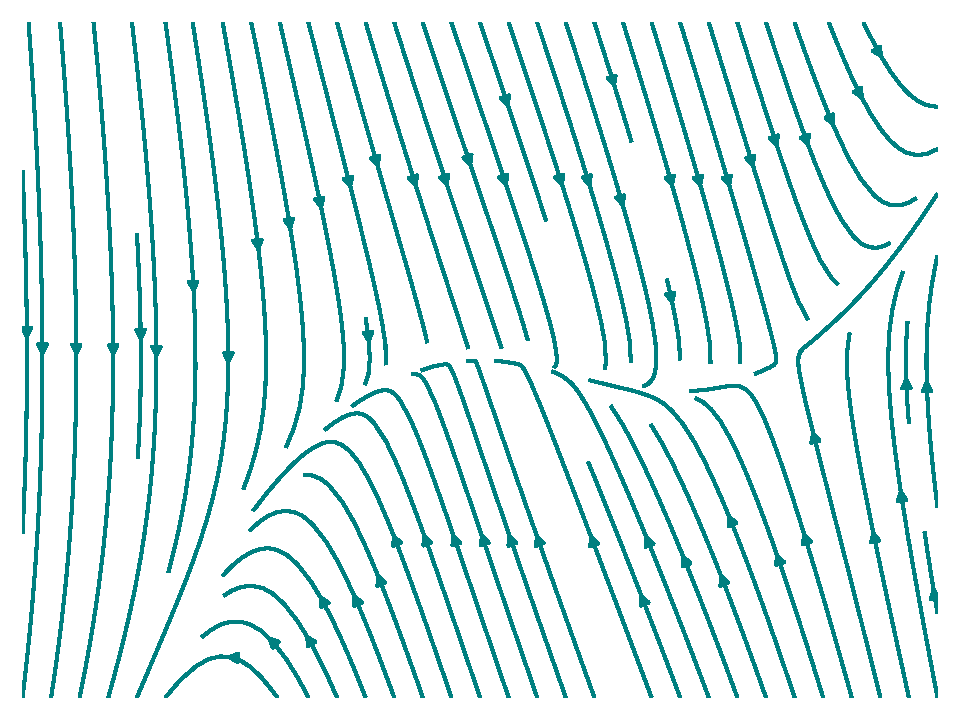
\includegraphics[width=7cm]{sistema com 2theta.pdf}
	\end{figure}
	%

























	\section*{15/07/2022 --- Controle por Lyapunov}
\markboth{Controle por Lyapunov}{15/07/2022}
\noindent\textbf{\sffamily Exercício 1.}
	Encontre um controle $u$ de Lyapunov que estabilize o pêndulo sem atrito,
	%
	\[
	    \ddot{x} = -\sin x + u,
	\] 
	%
	em $x=\pi/2$. \\

\noindent{\textbf{{\sffamily Exercício 2.}}
	Estabilize o sistema anterior no ponto $x=\pi/4$ com um novo controle mais inteligente.\\
	
\noindent{\textbf{{\sffamily Exercício 3.}}
	Proponha um sistema de controle por Lyapunov para o sistema dinâmico abaixo.
	%
	\[
		\frac{d^2\theta}{d\theta^2} = -2\theta 
		                              -4\frac{d\theta}{dt} 
		                              +\left(\frac{d\theta}{dt}\right)^{\!3}
		                              +u
	\]
	%
\noindent{\textbf{{\sffamily Exercício 4.}}
	Repita o exercício anterior trocando a parcela $-2\theta$ na EDO por $-2\theta^3$. \\
	
\noindent{\textbf{{\sffamily Exercício 5.}}
	Repita o exercício 3 trocando a parcela $-2\theta$ na EDO por $-2\theta^2$. \\
\rule{\textwidth}{0.5pt}\\

\noindent{\textbf{{\sffamily Exercício 1 --- solução.}} \\
	Pensando matematicamente, procuramos um ``equilíbrio deslocado", em comparação com os clássicos equilíbrios na origem.
	Pondo dessa maneira, faz sentido tentar $H$ de Lyapunov dada por 
	%
	\[
		H(x) = \frac{\dot{x}^2}{2} + 
		       \frac{\e}{2}\left(x-\frac{\pi}{2}\right)^2.
	\]
	%
	$\e>0$ é posto para garantir a positividade definida da função.
	Derivando, vem
	%
	\begin{align*}
		\dot{H} &= \dot{x}\ddot{x} + \e\left(x-\frac{\pi}{2}\right)\dot{x} \\
		        &= \dot{x}(\ddot{x} + \e\left(x-\frac{\pi}{2}\right)) \\
		        &= \dot{x}(-\sin x + \e\left(x-\frac{\pi}{2}\right) + u).
	\end{align*}
	%
	Logo, uma lei de controle que satisfaz $\dot{H}\leq 0$ é 
	$u = \sin x -\alpha\dot{x} - \e\left(x-\frac{\pi}{2}\right)$, $\alpha>0$. \\
	
\noindent{\textbf{{\sffamily Exercício 2 --- solução.}} \\
	Trocar $\pi/2$ por $\pi/4$ na $H$ acima resultaria no controle
	$u = \sin x -\alpha\dot{x} - \e\left(x-\frac{\pi}{4}\right)$, $\alpha>0$.
	
	O problema com tal $u$ é que pequenos distúrbios no ponto de equilíbrio são amplificados pelo seno antes de serem efetivamente reduzidos pelo ``atrito" $-\e x$.
	Esse comportamento é precisamente oposto ao da função cosseno, e por causa disso o objetivo será trocar na lei de controle original o seno pelo cosseno.
	
	Realizando a substituição, e a partir daí reconstruindo $H$, chegamos à seguinte expressão:
	%
	\begin{align*}
		\dot{H} &= \dot{x}(u-\cos x +\e\left(x-\frac{\pi}{4}\right)) \\ 
		        &= \dot{x} (\ddot{x} + \sin x - \cos x 
		                   + \e\left(x-\frac{\pi}{4}\right)) \\
		        &= \dot{x}\sqrt{2}\sin\left(x-\frac{\pi}{4}\right) +
		           \dot{x}\e\left(x-\frac{\pi}{4}\right) +
		           \dot{x}\ddot{x} \\
		\implies
		H(\theta) &= \sqrt{2}(c_1 - \cos\left(x-\frac{\pi}{4}\right)) +
		             \frac{\e}{2}\left(x-\frac{\pi}{4}\right)^2 +
		             \frac{\dot{x}^2}{2}.
	\end{align*}
	%
	Escolhendo $c_1=1$, $H$ acima se torna positiva definida com derivada $\leq0$ através do controle proposto, e o problema está fechado. \\
	%
	\begin{figure}[H]\centering
		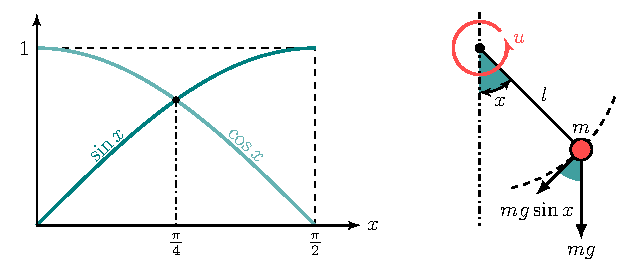
\includegraphics{sen vs cos.pdf}
		\caption{%
			Quando $x=\pi/4+\delta$, $u$ com $\sin x$ aumenta, distanciando o pêndulo do equilíbrio, enquanto $u$ com $\cos x$ diminui, facilitando a volta ao equilíbrio pela força peso.
			Quando $x=\pi/4-\delta$, $u$ com $\cos x$ aumenta para compensar a força peso, enquanto $\sin x$ relaxa, novamente distanciando o pêndulo do equilíbrio.
		}
	\end{figure}
	
\noindent{\textbf{{\sffamily Exercício 3 --- solução.}}\\
	Aqui vale tomar $H$ como a consagrada combinação linear entre $\theta$ e suas derivadas. Por exemplo, considere
	%
	\[
		H(\theta) = \frac{\dot{\theta}^2}{2} + 2\frac{\theta^2}{2}.
	\]
	%
	Perceba que a função acima é positiva definida. 
	Derivando-a no tempo, temos
	%
	\begin{align*}
		\dot{H} &= \dot{\theta}\ddot{\theta} + 2\theta\dot{\theta} \\
		        &= \dot{\theta}(\ddot{\theta} + 2\theta) \\
		        &= \dot{\theta}(-4\dot{\theta} + \dot{\theta}^3 + u),
	\end{align*}
	%
	de maneira que, para obter $\dot{H} \leq 0$, podemos escolher por exemplo 
	$u = -\dot{\theta}^3$. 
	
	De fato, tal $u$ nos leva a $\dot{H} = -4\dot{\theta}^2 \leq 0$. \\
	
\noindent{\textbf{{\sffamily Exercício 4 --- solução.}}\\
	Fisicamente, tanto $-2\theta$ quanto $-2\theta^3$ podem ser interpretados como coeficientes de atrito à variação de $\theta$, de forma que o novo sistema continua estável como o original. 
	
	Entretanto, tomar $H$ como no exercício anterior levaria a uma lei de controle talvez demasiadamente carregada, e assim o desafio aqui será definir $H$ que dê o mesmo $u$ anterior. 
	Conseguimos isso incluindo na função de Lyapunov a integral (em $\theta$) da parcela nova:
	%
	\begin{align*}
		H(\theta) = \frac{\dot{\theta}^2}{2} + 2\frac{\theta^4}{4} 
		\implies
		\dot{H} &= \dot{\theta}\ddot{\theta} + 2\theta^3\dot{\theta} \\
		        &= \dot{\theta}(\ddot{\theta} + 2\theta^3) \\
		        &= \dot{\theta}(-4\dot{\theta} + \dot{\theta}^3 + u) 
		        \leq 0
		\implies u = -\dot{\theta}^3,
	\end{align*}
	%
	como desejávamos. \\

\noindent{\textbf{{\sffamily Exercício 5 --- solução.}}\\
	Ao contrário dos problemas anteriores, a nova parcela não pode mais ser entendida como um atrito, e sua integral em $\theta$ não é positiva definida. 
	Para nos livrarmos desse empecilho, tentativamente tomamos
	%
	\[
		H(\theta) = \frac{\dot{\theta}^2}{2} +
		            2\frac{\theta^2|\theta|}{3},
	\]
	%
	de forma que, para $\theta\geq0$,
	%
	\begin{flalign*}
		\dot{H} &= \dot{\theta}\ddot{\theta} + 2\theta^2\dot{\theta} & \\
		        &= \dot{\theta}(\ddot{\theta} + 2\theta^2) \\
		        &= \dot{\theta}(-4\dot{\theta} + \dot{\theta}^3 + u) 
		        \leq 0
		\implies
		u = -\dot{\theta}^3,
	\end{flalign*}
	%
	e para $\theta<0$,
	%
	\begin{flalign*}
		\dot{H} &= \dot{\theta}\ddot{\theta} - 2\theta^2\dot{\theta} & \\
		        &= \dot{\theta}(\ddot{\theta} - 2\theta^2) \\
		        &= \dot{\theta}(-4\dot{\theta} - 4\theta^2 + \dot{\theta}^3 + u) 
		        \leq 0
		\implies
		u = -\dot{\theta}^3 + 4\theta^2.
	\end{flalign*}
	%
	Unindo as leis de controle numa única equação, ficamos com 
	$u(t) = -\dot{\theta}^3 + 2\theta(\theta - |\theta|)$.
	 
	\section*{22/07/2022 --- Introdução a saídas planas}
\markboth{Introdução a saídas planas}{22/07/2022}
\noindent\textbf{\sffamily Exercício 1.}\\
	Dado uma trajetória polinomial $x(t)$ tal que 
	%
	\[
		x(0) = \dot{x}(0) = \ddot{x}(0) 
		     = \dot{x}(10)= \ddot{x}(10)
		\quad\text{ e }\quad
		x(10) = 1,
	\]
	% 
	encontre $u$ que satisfaça 
	%
	\[
		\ddot{x} = -\sin(x-u).
	\]
	%
	\rule{\textwidth}{0.5pt}\\

\noindent\textbf{\sffamily Exercício 1 --- solução.}\\
	Exitem $6$ equações acerca de $x(t)$, de foma que este é polinômio de ordem $5$ ou maior. 
	Tomemos $x$ de grau 5 genérico, i.e., com $c_i$, $0\leq i\leq 5$, tais que
	%
	\[
		x(t) = c_0 + c_1t + c_2t^2 + c_3t^3 + c_4t^4 + c_5t^5
	\]
	%
	satisfaça às equações no enunciado. Substituindo, temos
	%
	\begin{align*}
		\left\{
			\begin{array}{rl}
				0 &= x(0)         \\ 
				0 &= \dot{x}(0)   \\ 
				0 &= \ddot{x}(0)  \\ 
				0 &= \dot{x}(10)  \\ 
				0 &= \ddot{x}(10) \\ 
				1 &= x(10)     
			\end{array}
		\right.
		\implies
		\left\{
			\begin{array}{rl}
				0 &= c_0 \\ 
				0 &= c_1 \\ 
				0 &= c_2 \\ 
				0 &= 3\cdot 10^2c_3 + 4\cdot 10^3 c_4 + 5\cdot 10^4 c_5 \\ 
				0 &= 6\cdot 10c_3 + 12\cdot 10^2 c_4 + 20\cdot 10^3 c_5 \\ 
				1 &= 10^3c_3 + 10^4c_4 + 10^5c_5 
			\end{array}
		\right.
		\implies
		\begin{pmatrix} 
			c_0 \\ c_1 \\ c_2 \\ c_3 \\ c_4 \\ c_5
		\end{pmatrix}
		= 
		\begin{pmatrix} 
			0 \\ 0 \\ 0 \\ 1/100 \\ -3/2000 \\ 3/50000
		\end{pmatrix}.
	\end{align*}
	%
	Conclui-se então que
	%
	\[
		u(t) = \arcsin(\ddot{x}(t)) + x(t)
		     = \arcsin\left(
		     	   \frac{6}{100}t - \frac{36}{2000}t^2 + \frac{60}{50000}t^3 
		       \right)
		       +
		       \frac{1}{100}t^3 - \frac{3}{2000}t^4 +\frac{3}{50000}t^5.
	\]
	%
	\begin{figure}[H]\centering
		\includegraphics{trajetória x.pdf}
		\caption{Gráfico em escala de $x(t)$ para $0\leq t\leq1$.}
	\end{figure}



	\section*{29/07/2022 --- SBPC}
\markboth{SBPC}{29/07/2022}
	Não houve aula.
	\section*{05/08/2022 --- Prova 1}
\markboth{Prova 1}{05/08/2022}
%	
	\textbf{\sffamily Questões}
	\begin{enumerate}
		\item [1)]
		Considerando os sistemas abaixo trace o retrato de fase dos mesmos e defina seus tipos.
		%
		\begin{itemize}
			\item [a)] 
			$\dis \frac{d^2 x}{dt^2} = 2x - \frac{dx}{dt} + u$
			{\hfill \tt (1.5)}
			
			\item [b)]			
			$\dis \frac{d^2 x}{dt^2} = -2x + \frac{dx}{dt} + u$
			{\hfill \tt (1.5)}
		\end{itemize}
		
		\item [2)]
		Considerando o sistema abaixo, determine o(s) ponto(s) de equilíbrio do mesmo e o(s) sistema(s) linearizado(s) tangente(s) associado(s).
		{\hfill \tt (3.0)}
		%
		\begin{align*}
			\frac{dx_1}{dt} &= -x_1(1-2x_2^2) - x_2 + ux_1 \\
			\frac{dx_2}{dt} &= x_1 - 1
		\end{align*}
		
		\item [3)]
		Determine uma função de Lyapunov e sua região de estabilidade do sistema abaixo. 
		{\hfill \tt (2.0)} \\
		Proponha um controle por Lyapunov para melhorar a performance do sistema 
		{\hfill \tt (2.0)}
		%
		\[
			\frac{d^2x}{dt^2} = -x - \frac{dx}{dt} + 
			                    \left(\frac{dx}{dt}\right)^3 + u + 1
		\]	
		%
	\end{enumerate}
	\rule{\textwidth}{0.5pt} \\
	\textbf{\sffamily Soluções}
	\begin{enumerate}
		\item [1)]
		Tomando a clássica escolha de estados $x_1=x$, $x_2=\dot{x}$, temos  para o sistema (a)
		%
		\[
			\dot{X} 
			= 
			AX + BU
			=
			\begin{pmatrix} 
				0 & 1 \\ 
				2 & -1 
			\end{pmatrix}
			X +
			\begin{pmatrix} 1 \\ 0 \end{pmatrix} u.
		\]
		%
		\textbf{Calculando os autovalores}
		\begin{align*}
			0 = \det(\lambda\I - A)         \iff 
			0 &= \lambda(\lambda+1) - 2  \\ \iff
			0 &= \lambda^2 + \lambda - 2 \\ \iff
			\lambda &= \lambda_1 = 1 \quad\vee\quad
			\lambda = \lambda_2 = -2.
		\end{align*}
		
		\textbf{Calculando os autovetores}
		\begin{align*}
			Av_1 &= \lambda_1 v_1 \iff 
			v_1 = x\begin{pmatrix} 1 & 1 \end{pmatrix}^T, 
			\quad\,\,\,\, x\in\R \\
			%
			Av_2 &= \lambda_1 v_2 \iff 
			v_2 = y\begin{pmatrix} 1 & -2 \end{pmatrix}^T, \quad y\in\R
		\end{align*}
	
		\textbf{Esboço do retrato de fase} \\
		Como $\lambda_2 < 0 < \lambda_1$, o RF será uma sela, e mais do que isso, os autovetores nos dizem que essa sela tem eixo instável na reta $x_2=x_1$ e estável na reta $x_2=-2x_1$.
		Segue o esboço.
		%
		\begin{figure}[H]\centering
			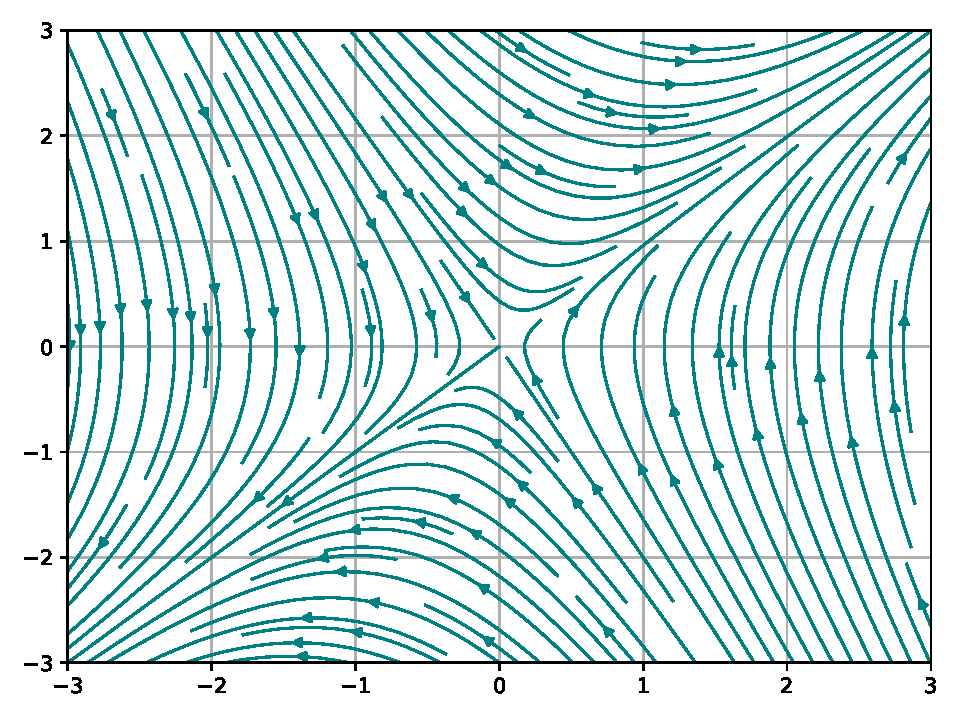
\includegraphics[width=7cm] {sela da prova1.pdf}
		\end{figure}
		%
		Para o sistema (b), 
		$A = 
		\begin{pmatrix} 
			0 & 1 \\
			-2 & 2
		\end{pmatrix}.$ \\
		
		\textbf{Calculando os autovalores}
		\begin{align*}
			0 = \det(\lambda\I - A)          \iff 
			0 &= \lambda(\lambda-2) + 2   \\ \iff
			0 &= \lambda^2 - 2\lambda + 2 \\ \iff
			\lambda &= \lambda_1 = 1+i \quad\vee\quad
			\lambda  = \lambda_2 = 1-i.
		\end{align*}
		%		
		\textbf{Esboço do retrato de fase} \\
		Como $\Re(\lambda_{1,2}) > 0$, o RF será um foco instável.
		Segue o esboço.
		%
		\begin{figure}[H]\centering
			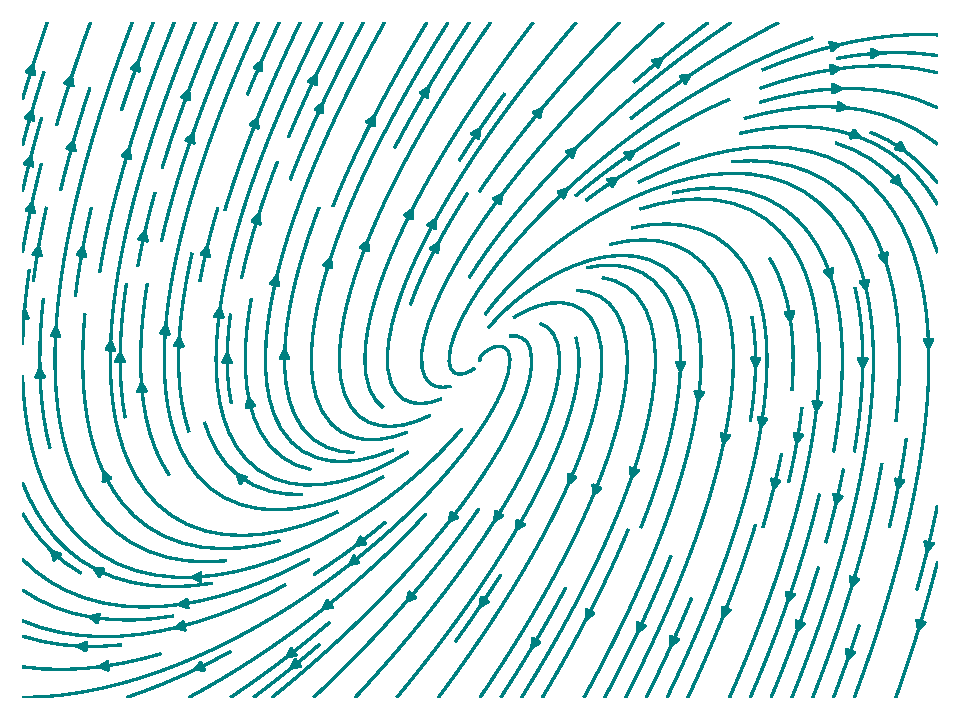
\includegraphics[width=7cm] {foco da prova1.pdf}
		\end{figure}
		%
		
		\item [2)]
		No ponto de equilíbrio $(\bar{x_1}, \bar{x_2})$, 
		$\dot{x}_1 = \dot{x}_2 = u = \bar{u} = 0$. 
		Substituindo nas EDOs, vem 
		%
		\begin{align*}
			\left\{	
				\begin{array}{l}
					0 = -\bar{x_1}(1 - 2\bar{x_2}^2) - \bar{x_2} \\
					0 = \bar{x_1} - 1
				\end{array}
			\right.
			\implies 
			\bar{x_1} = 1, \quad 2\bar{x_2}^2 - \bar{x_2} - 1.
		\end{align*}
		%
		Resolvendo a quadrática, chegamos a dois possíveis pontos de equilíbrio: 
		$P_1 = (1, 1)^T$ e $P_2 = (1, -1/2)^T$.
		Prosseguindo, linearizamos 
		$f_1(X;u) := \dot{x}_1$ e 
		$f_2(X;u) := \dot{x}_2$.
		Veja que
		%
		\[
			\begin{array}{lll}				
				\del_{x_1}f_1|_{(\bar{x_1}, \bar{x_2})}
				= 2\bar{x_2}^2-1  
				&
				\del_{x_2}f_1|_{(\bar{x_1}, \bar{x_2}) }
				= 4\bar{x_1x_2}-1
				&
				\del_u f_1|_{(\bar{x_1}, \bar{x_2})}
				= \bar{x_1} 
				\\
				\del_{x_1}f_2|_{(\bar{x_1}, \bar{x_2})}
				= 1 
				&
				\del_{x_2}f_2|_{(\bar{x_1}, \bar{x_2}) }
				= 0
				&
				\del_u f_2|_{(\bar{x_1}, \bar{x_2})}
				= 0 
			\end{array}
		\]
		%
		e portanto o linearizado em cada $P_j$ fica
		%
		\begin{align*}
			(\bar{x_1}, \bar{x_2}) = P_1 \implies
			\dot{X} &= 
			\begin{pmatrix} 
				1 & 3 \\ 1 & 0
			\end{pmatrix}
			(X-P_1) +
			\begin{pmatrix} 
				1 \\ 0
			\end{pmatrix}
			u,
			\\
			(\bar{x_1}, \bar{x_2}) = P_2 \implies
			\dot{X} &= 
			\begin{pmatrix} 
				-1/2 & -3 \\ 1 & 0
			\end{pmatrix}
			(X-P_2) +
			\begin{pmatrix} 
				1 \\ 0
			\end{pmatrix}
			u.
		\end{align*}
		
		\item [3)]
		Primeiro estabelecemos a estabilidade do sistema. Como este tem ponto de emquilíbrio $(x, \dot{x}) = (1, 0)$, tentamos $H$ de Lyapunov dada por 
		%
		\begin{equation}
			H(x(t)) = \frac{(x-1)^2}{2} + \frac{\dot{x}^2}{2}.
			\label{H da prova}
		\end{equation}
		%
		É fácil ver que $H$ acima é positiva para os pontos diferentes do equilíbrio e nula nele.
		O próximo passo é verificar a derivada de $H$ do tempo; temos
		%
		\begin{align*}
			\dot{H} &= \dot{x}(x-1) + \dot{x}\ddot{x} \\
			        &= \dot{x}(x-1+\ddot{x}) \\
			        &= \dot{x}(-\dot{x}+\dot{x}^3),
		\end{align*}
		%
		função nula no equilíbrio mas não necessariamente negativa fora dele. 
		Assim sendo, procuremos saber a região onde a estabilidade é garantida, isto é, $\dot{H}<0$ com $\dot{x}\neq 0$. 
		Vem
		%
		\begin{align*}
			\dot{x}(-\dot{x}+\dot{x}^3) < 0 \iff
			\dot{x}^2(\dot{x}^2-1) < 0      \iff
			\dot{x}^2-1 < 0                 \quad\therefore\quad
			0<|\dot{x}|<1.
		\end{align*}
		%
		A inequação acima define a região de estabilidade. 
		O retrato de fase do sistema mosrta que, realmente, esse intervalo abrange quase toda a região estável do sistema, embora não seja condição suficiente para a estabilidade.
		%
		\begin{figure}[H]\centering
			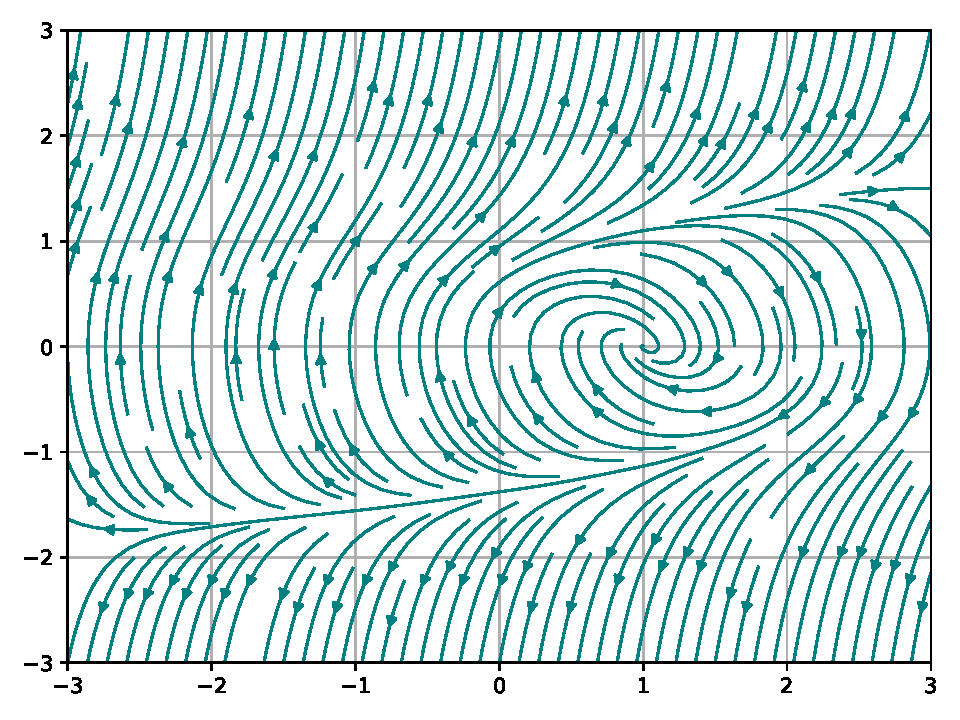
\includegraphics[width=7cm]{sistema de Lyapunov da prova1.pdf}
		\end{figure}
		%
		Agora, propomos controle de Lyapunov. Tomando a mesma $H$ de \eqref{H da prova}, a derivada se torna 
		%
		\begin{align*}
			\dot{H} &= \dot{x}(x - 1 + \ddot{x}) \\
			        &= \dot{x}(-\dot{x} + \dot{x}^3 + u),
		\end{align*}
		%
		e está claro que $u=-\dot{x}^3$, por exemplo, estabilizaria globalmente o sistema, melhorando sua performance.
	\end{enumerate}




















	%\include{Anotações/12-08-2022.tex} % ?
	%\include{Anotações/19-08-2022.tex} % inicio de flatness de fato
	%\include{Anotações/26-08-2022.tex} % aula com o Oniram
	%\include{Anotações/02-09-2022.tex} % aula amanhã
	%
	%\include{Anotações/19-08-2022.tex}
	
	
\end{document}